\documentclass[a4paper]{article}

\usepackage[utf8]{inputenc}
\usepackage[T1]{fontenc}
\usepackage[italian]{babel}

\usepackage{siunitx}
\usepackage{amsmath}
\usepackage{amssymb}
\usepackage{hyperref}
\usepackage{graphicx}
\usepackage[font={sf}]{caption}

\setlength{\marginparwidth}{95pt}

\newcommand*\de{\mathrm{d}}

\title{Relazione laboratorio particelle\\Esperienza 0 (preliminare)}
\author{Andrea Marasciulli\\
Giacomo Petrillo\\
Roberto Ribatti}
\date{Dal 13 al 19 novembre 2017\footnote{Compilazione \LaTeX{} di questo documento: \today.}}

\begin{document}
	
\maketitle

\marginpar{punto 1}

Scegliamo di usare, in ordine dal basso verso l'alto, i PMT 2, 3, 4.

\marginpar{punto 2}

Accendiamo il PMT~2 a \SI{1500}V.

\marginpar{punto 3}

Schizzo dei segnali del PMT visti sull'oscilloscopio:

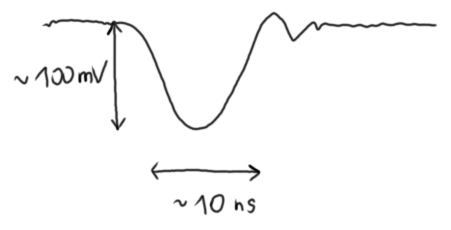
\includegraphics[width=9cm]{fig3a}

Con il trigger a \SI{-27}{mV}, contando a mano su \SI1{min}, otteniamo $\sim\SI1{Hz}$.

\subsection*{Amplificazione}

Stimiamo l'energia rilasciata da una particella nello scintillatore.
Supponiamo MIP, quindi
$\de E/\rho\de x=\SI{1.5}{MeV\,g^{-1}\,cm^2}$.
Lo spessore dello scintillatore è $\sim\SI1\cm$ e la densità $\sim\SI1{g\,cm^{-3}}$,
quindi rilascia $\SI{1.5}{MeV} = \SI{2.4e-13}{J}$.

Stimiamo l'energia del segnale in uscita. È
$\int\de t\, I\cdot V \approx \Delta t\cdot V^2/R$
dove $R=\SI{50}\ohm$, quindi otteniamo
$\num{10e-9}\cdot(\num{100e-3})^2/50=\SI{2e-12}{J}$.

L'amplificazione complessiva è quindi $\sim10$, a naso ce la aspettavamo più grande.

\subsection*{Dipendenza rate dall'alimentazione}

Impostiamo la tensione di alimentazione a \SI{1600}V.
La frequenza di segnali aumenta notevolmente,
per contarli a mano alziamo\footnote{Trattando la logica negativa, useremo alto-basso riferito al modulo e spesso tralasceremo il segno $-$,  la strumentazione suggerisce questo approccio perché la vite della soglia del discriminatore aumenta (abbassa) la soglia in verso orario.} il trigger a \SI{150}{mV},
otteniamo $85/\SI1{min}$.

Con \SI{1800}V otteniamo $\sim\SI{100}{Hz}$ e con \SI{2000}V $\sim\SI{1}{kHz}$
(frequenze misurate dall'oscilloscopio).

\marginpar{punto 4}

\subsection*{Documentazione discriminatore}

Non troviamo la documentazione del nostro discriminatore tra quella fornita;
poiché è a 4 canali e l'unica documentazione per uno a quattro canali è il CAEN~N84,
e inoltre a parte colore e etichette appare identico,
leggiamo la documentazione per quello e chiameremo il nostro <<N84>>.

Documentazione:
ritardo \SI{14}{ns},
durata 6--400\,\si{ns},
soglia massima \SI{400}{mV}.

\subsection*{Verifica discriminatore}

Montiamo questo circuito:

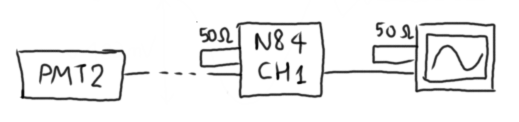
\includegraphics[width=9cm]{fig4a}

Girando la vite della durata vediamo che l'intervallo impostabile è circa 40--300\si{\,ns}.
È di tipo ``restarting'' perché per soglia abbastanza bassa si vedono durate doppie in uscita,
con soglia a opportuni valori intermedi si vedono alternativamente durate doppie oppure due singole, ravvicinate ma non più di tanto.
L'ampiezza è \SI{750}{mV} come atteso.
Verifichiamo la durata impostabile anche per il canale~2, è la stessa.

Modifichiamo il circuito in modo da visualizzare sia l'ingresso che l'uscita del discriminatore:

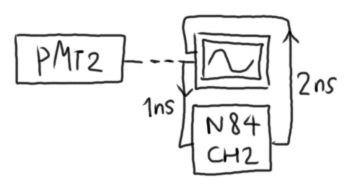
\includegraphics[width=5cm]{fig4b}

Misuriamo la soglia del discriminatore con l'oscilloscopio in questo modo:
triggeriamo sull'ingresso del discriminatore,
se la soglia del discriminatore è minore di quella del trigger
si vede sempre l'uscita del discriminatore,
viceversa a volte scompare.
Trovando due soglie del trigger più vicini possibili in modo che con una a volte scompare l'uscita (verificato su un tempo abbastanza lungo rispetto alla differenza delle soglie) e con l'altra no, si ottiene una misura della soglia del discriminatore.
Il problema di questa procedura è che il trigger dell'oscilloscopio funziona in modo diverso dal discriminatore, quindi non è detto che a parità di soglia vengano selezionati gli stessi segnali.
Con la soglia del discriminatore al massimo otteniamo le soglie del trigger 368 e \SI{376}{mV},
mentre il TP del discriminatore segna \SI{0.411}V, quindi lo scarto è circa \SI8\percent.

Il ritardo è dato da quello dei cavi (\SI3{ns}) più quello del discriminatore.
Puntando i cursori dell'oscilloscopio otteniamo un ritardo di \SI{20}{ns}
quindi il ritardo del discriminatore è circa \SI{17}{ns}.

Ci è difficile misurare il jitter del discriminatore perché il trigger dell'oscilloscopio funziona in modo diverso dal discriminatore, perciò facciamo una stima superiore in questo modo:
mettiamo la soglia del trigger ai \SI{376}{mV} trovati prima che facevano circa coincidere i segnali selezionati, triggerando il segnale del PMT, e guardiamo a occhio sull'oscilloscopio la variazione temporale del fronte di salita dell'uscita del discriminatore; otteniamo \SI{\pm1}{ns}.

\marginpar{punto 5}

\subsection*{Documentazione contatore}

Modello: 130PCZ,
\marginpar{Siamo sicuri o era l'unico datasheet?}%
frequenza massima \SI{70}{MHz},
conta fino a $10^8-1$,
l'input deve durare almeno \SI7{ns},
l'output ``clock'' è un'onda quadra a \SI1{kHz}.
\marginpar{Qual è il duty del clock? \SI{50}\percent?}

\subsection*{Clock del contatore}

Si può collegare il clock all'ingresso~8 per misurare il tempo.
Si può impostare in modo che dopo $10^n$ $(n=2,\dots,8)$
\marginpar{o era $1,\dots,8$?}%
conteggi si fermi.
Se avviamo il conteggio con il pulsante <<start>> o con l'ingresso corrispondente
e lo facciamo fermare in automatico con il clock,
introduciamo un'incertezza sul tempo totale dovuta al non allineamento dello start con il clock\footnote{Potremmo darlo per ovvio, però notiamo che quasi sicuramente i comandi manuali/ingresso non vengono allineati dallo strumento con il fronte successivo del clock perché gli ingressi possono definire intervalli di tempo con molta più granularità di \SI1{ms}.}.
L'incertezza è circa di mezzo periodo, quindi \SI{.5}{ms}.

Visualizziamo il clock sull'oscilloscopio, che calcola una frequenza di \SI{0.99996}{kHz},
cioè la discrepanza è di \SI3s al giorno.
Non sappiamo in che proporzione i due strumenti contribuiscono all'incertezza.
\marginpar{Possiamo fare delle supposizioni?}

\subsection*{Primo test di conteggio}

Montiamo questo circuito:

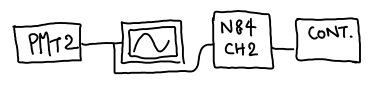
\includegraphics[width=9cm]{fig5a}

Il trigger dell'oscilloscopio è impostato a \SI{376}{mV}.
Mettiamo il clock a 1000 (\SI1s) e facciamo un po' di conteggi.
Il contatore gira intorno a 20;
la frequenza calcolata dall'oscilloscopio oscilla ampiamente perché probabilmente la calcola su intervalli di tempo piccoli rispetto al tasso di conteggi,
quando si stabilizza per qualche secondo gira intorno a \SI{30}{Hz},
quindi non troviamo incongruenze.

\subsection*{Distribuzione dei conteggi}

Ci aspettiamo che, per un tasso costante, i conteggi siano poissoniani con
$\text{media} = \text{tasso}\times \text{tempo}$.
Lo stimatore di massima verosimiglianza per la media è la media aritmetica ed è corretto\footnote{Unbiased.}.
La varianza dello stimatore è la media quindi,
con la convenzione standard di calcolare la varianza nella stima,
per $k$ conteggi il risultato per la media $\mu$ sarà scritto come
\[ \text{<<$\mu = k \pm \sqrt k$>>} \]
Questo è problematico per $k$ piccoli perché la varianza varia velocemente,
risolveremo nell'analisi dati.

\marginpar{punto 6}

\subsection*{Secondo test di conteggio}

Facciamo una serie di conteggi trascrivendo i risultati.
Facciamo 45 conteggi con clock 1000 e 15 con clock \num{10000}.
Verifichiamo che siano poissoniane con un test del $\chi^2$ senza allargare i bin rispetto ai valori discreti;
poiché il numero di conteggi è basso calcoliamo la distribuzione della statistica con monte carlo.
Risultati:

\noindent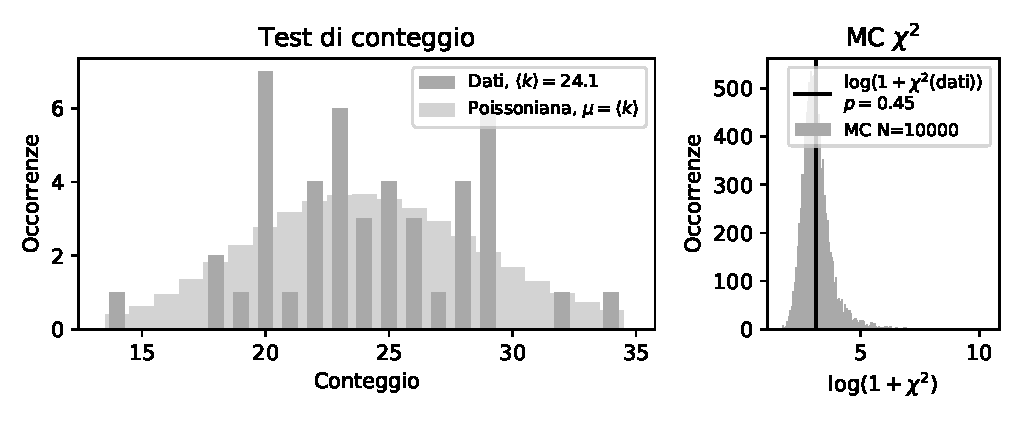
\includegraphics[width=\textwidth]{fig6a}

\noindent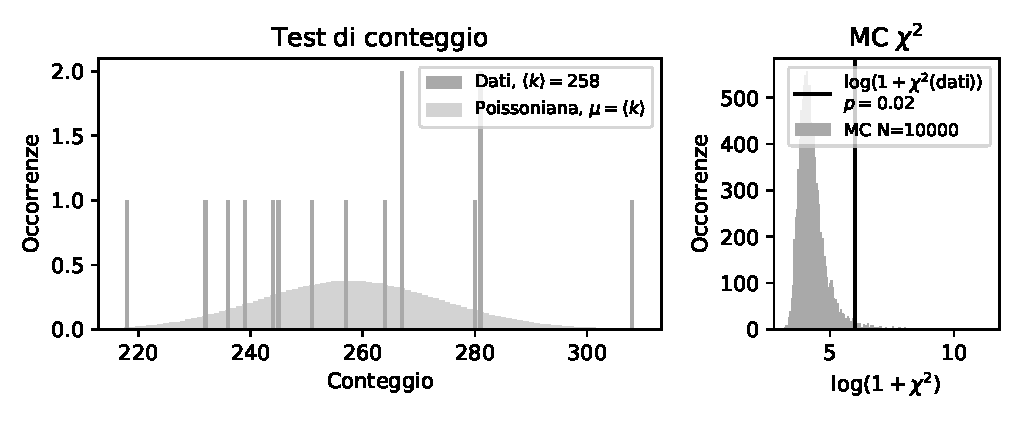
\includegraphics[width=\textwidth]{fig6b}

Vediamo che la poissonianietà della serie da \SI{10}s è in dubbio.

\subsection*{Tempo dall'accensione}

Può darsi che il PMT, dopo l'accensione, ci metta un po' ad arrivare in una condizione stazionaria di funzionamento.
I PMT 3 e 4 li abbiamo lasciati spenti, quindi li usiamo per fare un test.
Accendiamo il PMT~3 e subito prendiamo una serie di 15 conteggi con clock~1000.
Poi accendiamo il PMT~4 e prendiamo una serie, poi proseguiamo alternando PMT~3 e 4,
per un totale di 5 serie. Grafichiamo le medie con la varianza nell'ipotesi di poissoniane:

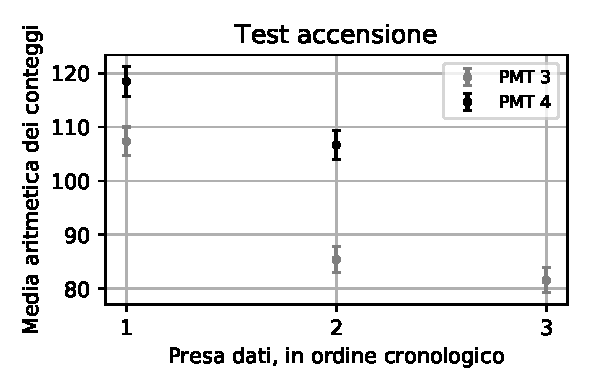
\includegraphics[width=7cm]{fig6c}

Chiaramente il tasso varia nel tempo, quindi in futuro aspetteremo sempre qualche minuto dopo che abbiamo acceso i PMT e almeno 1~minuto quando cambiamo tensione di alimentazione.

\subsection*{Luce ambientale}

Verifichiamo la sensibilità alla luce esterna passando una torcia vicino allo scintillatore e al PMT e verificando se il numero di conteggi cambia sensibilmente.
Testiamo i PMT 2, 3, 4.
\begin{center}
\begin{tabular}{c|p{50ex}}
	PMT & Risultato \\
	\hline
	4 &
	Troviamo un ``buco ottico'' sull'attacco della guida ottica al PMT,
	puntando la torcia i conteggi passano da $\approx 100$ a $\approx 200$. \\
	3 &
	Anche qui l'attacco del PMT alla guida ottica è problematico;
	la luce entra riflettendosi sulla base del PMT.
	I conteggi variano da $\approx 100$ a $\approx 280$.\\
	2 &
	Tutto ok.
\end{tabular}
\end{center}
Sistemiamo tutto con il nastro isolante e ricontrolliamo.

% -------------------------------------------


\subsection*{Alimentazione}

Abbiamo variato l'alimentazione dei vari PMT per vedere come cambia il numero di conteggi. I risultati di queste misure sono  riportati nel grafico di \emph{Figura \ref{tensio}}. 

\begin{figure}[h]
\centering
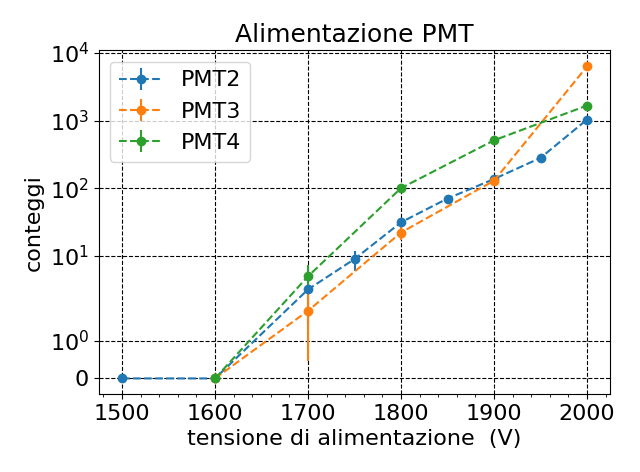
\includegraphics[width=8 cm]{tensio_pmt}
\caption{Numero di conteggi in funzione della tensione di alimentazione}
\label{tensio}
\end{figure}

Il grafico mostra chiaramente l'assenza di qualsiasi $plateau$ tranne nei punti a conteggio nullo. Abbiamo deciso di alimentare i PMT a 1800\! V perché la derivata in quel punto è minore di quella corrispondente a 1900\! V e ci sono abbastanza conteggi da permetterci una loro analisi statistica.

Dal \emph{Particle Physics Booklet 2016} sappiamo che il flusso di raggi cosmici è mediamente 180~Hz$/$\!m$^2$s. Essendo il nostro rivelatore di area $A=l_1l_2=48.0\pm0.1$\! cm $\cdot \, 40.0\pm0.1$\! cm$=1920\pm6$\! cm$^2$ ci aspettiamo il passaggio di 34.6$\pm$0.1 particelle$/$s. Questo numero è simile ai conteggi ottenuti a 1800\! V con soglia V$_{thr}\simeq-376$\! mV. 

\subsection*{Modulo di coincidenze}

Per effettuare il conteggio delle coincidenze abbiamo collegato le uscite dei discriminatori al modulo di coincidenze FE260 e la sua uscita al canale 5 dello scaler. I canali 1 e 2 di quest'ultimo sono collegati al PMT4 e al PMT2 attraverso il discriminatore. Le soglie di entrambi sono massime, ovvero $-0.410\pm0.002$\! V misurate dal testpoint. Con questi settaggi i nostri rivelatori misurano circa 40 eventi al secondo, quindi facciamo un calcolo approssimativo del rate di coincidenze casuali usando la formula $R_C=R_1R_2\Delta t$. Siccome il modulo di coincidenze scatta quando c'è una sovrapposizione  di due segnali di livello 1 per più di 1.5\! ns, possiamo dire che il $\Delta t$ vale circa il doppio della durata dell'uscita del discriminatore, ovvero 80\! ns. Abbiamo allora $R_C\simeq 128\cdot10^{-6}\approx1\cdot10^{-4}$, ovvero una coincidenza casuale ogni 3 ore.

\subsection*{Tempi di propagazione dei segnali}

Usiamo l'oscilloscopio per visualizzare le coincidenze, ovvero colleghiamo i due discriminatori utilizzati al nostro strumento ed osserviamo degli impulsi NIM quasi simultanei, in particolare vediamo che il segnale che arriva più tardi si discosta solo di qualche nanosecondo da quello precedente, ma questa asincronia non ci causa nessun problema perché vale al massimo il 10\% della lunghezza dei nostri impulsi.
% chiedere a Giacomo se ha già scritto perché abbiamo scelto l'ampiezza massima 
Ciò non dovrebbe mascherare l'arrivo di una seconda coincidenza in quell'intervallo di tempo perché il rate atteso è di decine di hertz, come già detto nella sezione \textbf{calibrazione}, che equivale in media al passaggio di un raggio cosmico ogni decimo di secondo in caso di accettanza geometrica unitaria.

Per trovare il miglior punto di lavoro inseriamo nel crate due \emph{delay unit} che colleghiamo in serie ai discriminatori di cui sopra. Prima di effettuare i conteggi testiamo una delay unit mandandole in ingresso l'onda quadra data dal clock dello scaler. Confermiamo che il ritardo minimo introdotto da questo modulo è 2.5$\pm$0.2\! ns e che tutti gli altri inseribili sono compatibili con quanto dichiarato con un'accuratezza del 10\%. La \emph{Figura \ref{curv}} mostra la curva di cavo che, come atteso, mostra un massimo di conteggi quando il ritardo relativo è inferiore alla durata dell'impulso del discriminatore ed è quasi nulla altrove. La variabile utilizzata è $\Delta t=D2-D4$ dove questi ultimi sono i ritardi selezionati per i rispettivi PMT. Nel $\Delta t$ non compaiono termini dipendenti dai cavi coassiali utilizzati perché i due segnali sono stati collegati ai vari moduli NIM con cavi di uguale lunghezza.

\begin{figure}[h]
\centering
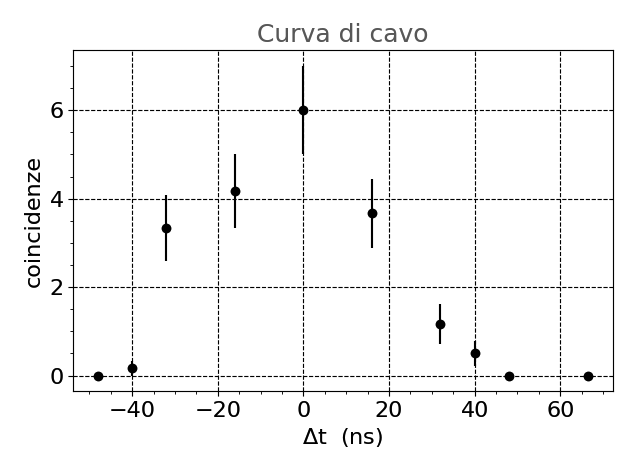
\includegraphics[width=8 cm]{curva_cavo}
\caption{Curva di cavo in funzione della differenza di tempi impostati sulle delay unit.}
\label{curv}
\end{figure}

% aggiungere il disegno di Giacomuzzo?


\subsection*{Rapporto segnale/fondo}

Dopo aver tolto le delay unit abbiamo variato la tensione di un PMT  e la soglia del discriminatore a cui era collegato mentre l'altro era lasciato ad un punto di lavoro costante in modo che non influenzasse le misure fatte sul primo. Abbiamo analizzato dapprima il PMT2 lasciando fisso il 4 ad una tensione nominale V$_4=1800$\! V ed una soglia V$_{thr_4}=-353\pm2$\! mV in modo che le concidenze casuali non potessero verificarsi in un intervallo di tempo di 10\! s. 
Il rapporto tra le coincidenze ed i conteggi rappresenta il rapporto tra segnale e segnale più rumore, in quanto il numero mostrato dallo scaler comprende sia i disturbi che le particelle. Il risultato è visibile in \emph{Figura \ref{test1}}.

\begin{figure}[h]
\centering
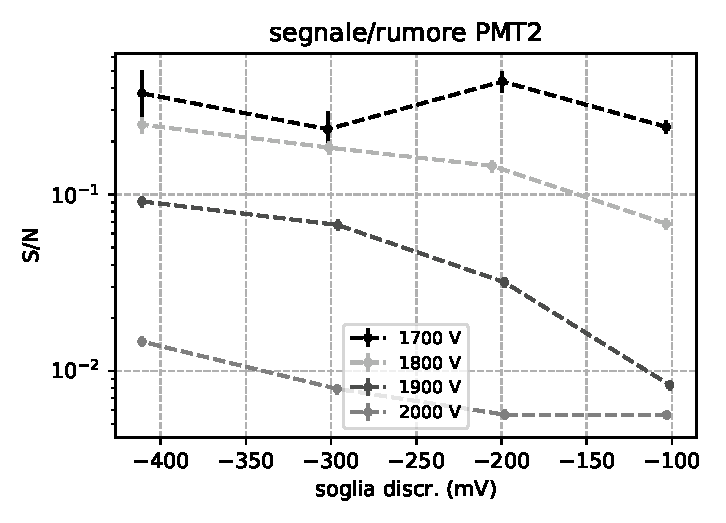
\includegraphics[width=8 cm]{calib_pmt2}
\caption{Rapporti S/(S+N) per il PMT2 in diversi punti di lavoro.}
\label{test1}
\end{figure}

La stessa cosa è stata fatta per il PMT4 lasciando il PMT2 al punto di lavoro V$_2=1820$\! V e V$_{thr_2}=-298\pm2$\! mV come mostrato in \emph{Figura \ref{test2}}.

\begin{figure}[h]
\centering
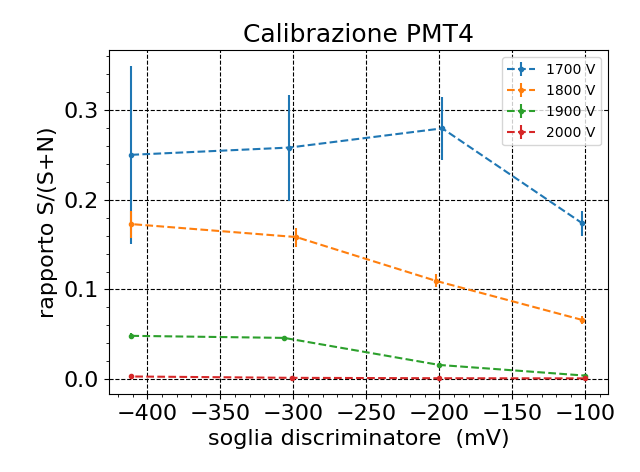
\includegraphics[width=8 cm]{calib_pmt4}
\caption{Rapporti S/(S+N) per il PMT4 in diversi punti di lavoro.}
\label{test2}
\end{figure}

\subsection*{Efficienza assoluta}

Per misurare l'efficienza assoluta del PMT3 è necessario eseguire i rapporti tra le coincidenze di tutti i tre rivelatori e quelle dei due più esterni. Per fare ciò abbiamo usato un secondo modulo di coincidenze per visualizzare quelle di tutti e tre. Non avendo ancora analizzato i dati riguardanti la sezione precedente, abbiamo stimato il punto di lavoro V$=1800$\! mV e V$_{thr}=-200$\! mV essere il migliore per i fotomoltiplicatori esterni. Quindi abbiamo variato soglia e alimentazione di quello centrale e disegnato il grafico di \emph{Figura \ref{eff}} per varie tensioni di alimentazione.

\begin{figure}[h]
\centering
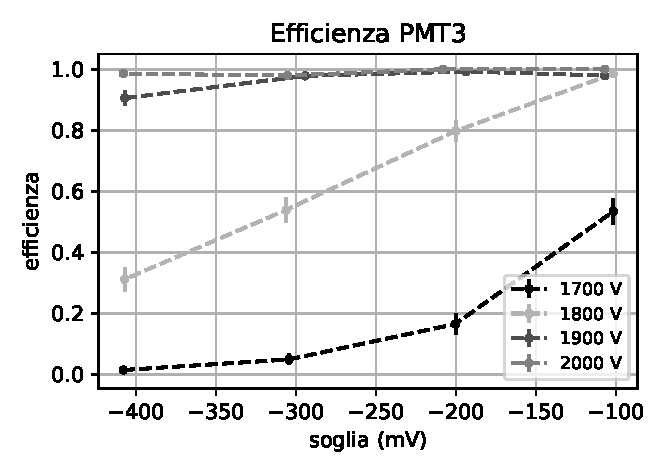
\includegraphics[width=8 cm]{efficienza}
\caption{\label{eff}Efficienza assoluta del PMT3.}
\end{figure}

L'analisi effettuata contrassegna il punto di lavoro scelto prima come migliore perché il PMT che lavora in quelle condizioni ha una buona efficienza ed anche un buon rapporto S$/$(S$+$N). Quest'ultimo ci permette di avere meno coincidenze casuali ed evita la possibilità di overflow in caso di conteggi su un tempo molto lungo. L'efficienza corrispondente a questo punto di lavoro vale $\eta=80\pm3$\! \%. Possiamo adesso determinare il rate di particelle cosmiche avvalendoci della relazione 
$$ R_V=\frac{R_m}{1+R_m\Delta t} $$
in cui R$_m$è il rate misurato, R$_V$ quello vero e $\Delta t$ stimato in precedenza. Essendo quest'ultimo dell'ordine dei nanosecondi, R$_m\Delta t \ll 1$. Il rate misurato si ottiene dividendo le coincidenze a 3 per l'efficienza. Nel punto di lavoro in questione abbiamo osservato Quindi il rate di raggi cosmici risulta essere R$_V=14\pm1$\! particelle$/$s. Esso è inferiore alla metà di quanto atteso ma ciò è dovuto all'accettanza geometrica minore di uno.

\end{document}
